\documentclass{article}
\usepackage{amsmath}
\usepackage{amssymb}
\usepackage{graphicx}
\usepackage{hyperref}
\usepackage[version=4]{mhchem}

\title{Example 1}
\date{}

\begin{document}
\maketitle

\(A B C\) is an isosceles triangle with \(A B=A C\). Circle \(O\) is drawn using \(A B\) as the diameter to intersect \(B C\) at \(D\). Show that \(B D=\) \(D C\).

Solution:
Connect \(O D\).\\
\centering
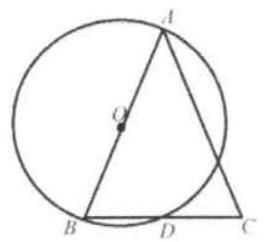
\includegraphics[width=\textwidth]{images/problem_image_1.jpg}

Since \(O B=O D\) (both are radius), \(\angle O B D=\angle O D B\).\\
Since \(A B=A C, \angle B=\angle C\).\\
So \(\angle A C B=\angle O D B\). Thus \(A C / / O D\).\\
Since \(B O=O A, B D=D C\).\\
\centering
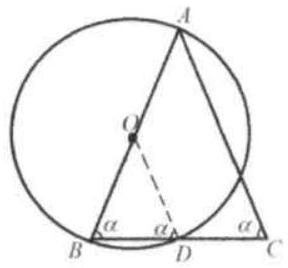
\includegraphics[width=\textwidth]{images/reasoning_image_1.jpg}


\end{document}
